\section{Games using Procedural Content Generation}
Procedural content generation is, as described previously, a powerful tool for generating content in games in ways that might not be possible to be created manually. PCG, however, is a broad concept and is utilized i many games i various ways. How a few of the more popular games utilizes PCG is described in this section. 

\subsection{Diablo}
\textit{Diablo} is a fantasy game about a group of warriors on a mission to hunt down the demon lord Diablo, who is threatening the village of Tristram. To reach Diablo in Hell, the player must go through a series of request that takes them on a journey through the difficult dungeon. \textit{Diablo} was likely a success because of its early on uses of PCG algorithms that randomly created dungeons for each new level. The developers used what they called a "Dynamic Random Level Generator" to generate a new dungeon for each level \cite{Diablo_PCG}. The generator provided a new gaming experience for the player every time the game was played. 

\begin{figure}[H]
    \centering
    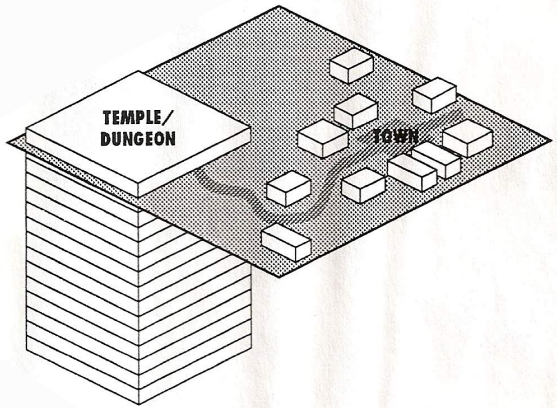
\includegraphics[width=0.5\linewidth]{Planning report/images/diablo.jpg}
    \caption{Level structure plan from the \textit{Diablo} pitch, the year 1994.}
    \label{fig:diablo_plan}
\end{figure}{}


\subsection{Minecraft}
\textit{Minecraft} is a popular game with a three-dimensional world consisting of cubes of earth, wood and other materials. The game is multi-functional, meaning that players can decide if they want to build structures and obtain objects from the world. There are environmental hazards that can kill players' avatars, but it is possible to avoid these in the game. \textit{Minecraft} is based on algorithms like Perlin Noise to generate unique terrains with large voxels~\cite{minecraft_PCG}. The game also uses Whittaker diagrams to determine what plants and other terrain features that should be added in different biomes. This makes the world more realistic, as seen in figure \ref{fig:biome}. As of May 2019, 10 years since its official release, \textit{Minecraft} has sold over 176 million copies~\cite{Minecraft_10ys}, proving its huge success.

\begin{figure}[H]
\centering
\begin{subfigure}{.48\linewidth}
  \centering
  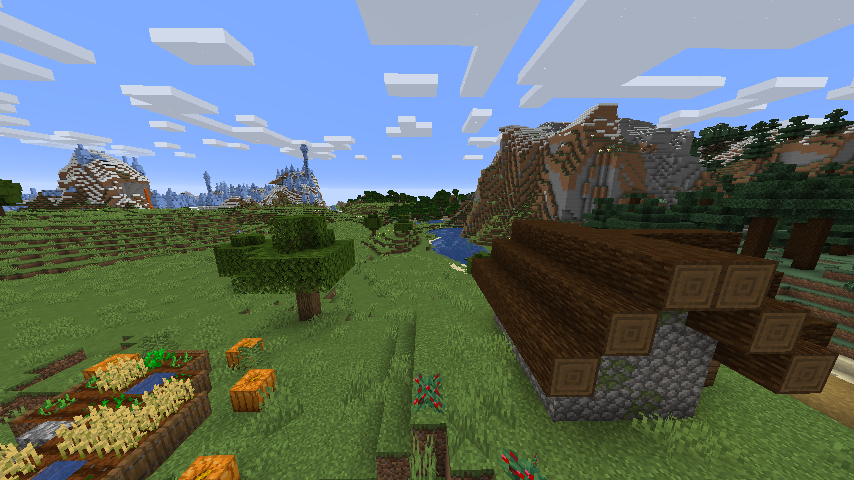
\includegraphics[width=1\linewidth]{Planning report/images/minecraft1.png}
  \caption{Minecraft world}
  \label{fig:minecraft}
\end{subfigure}
~
\begin{subfigure}{.48\linewidth}
  \centering
  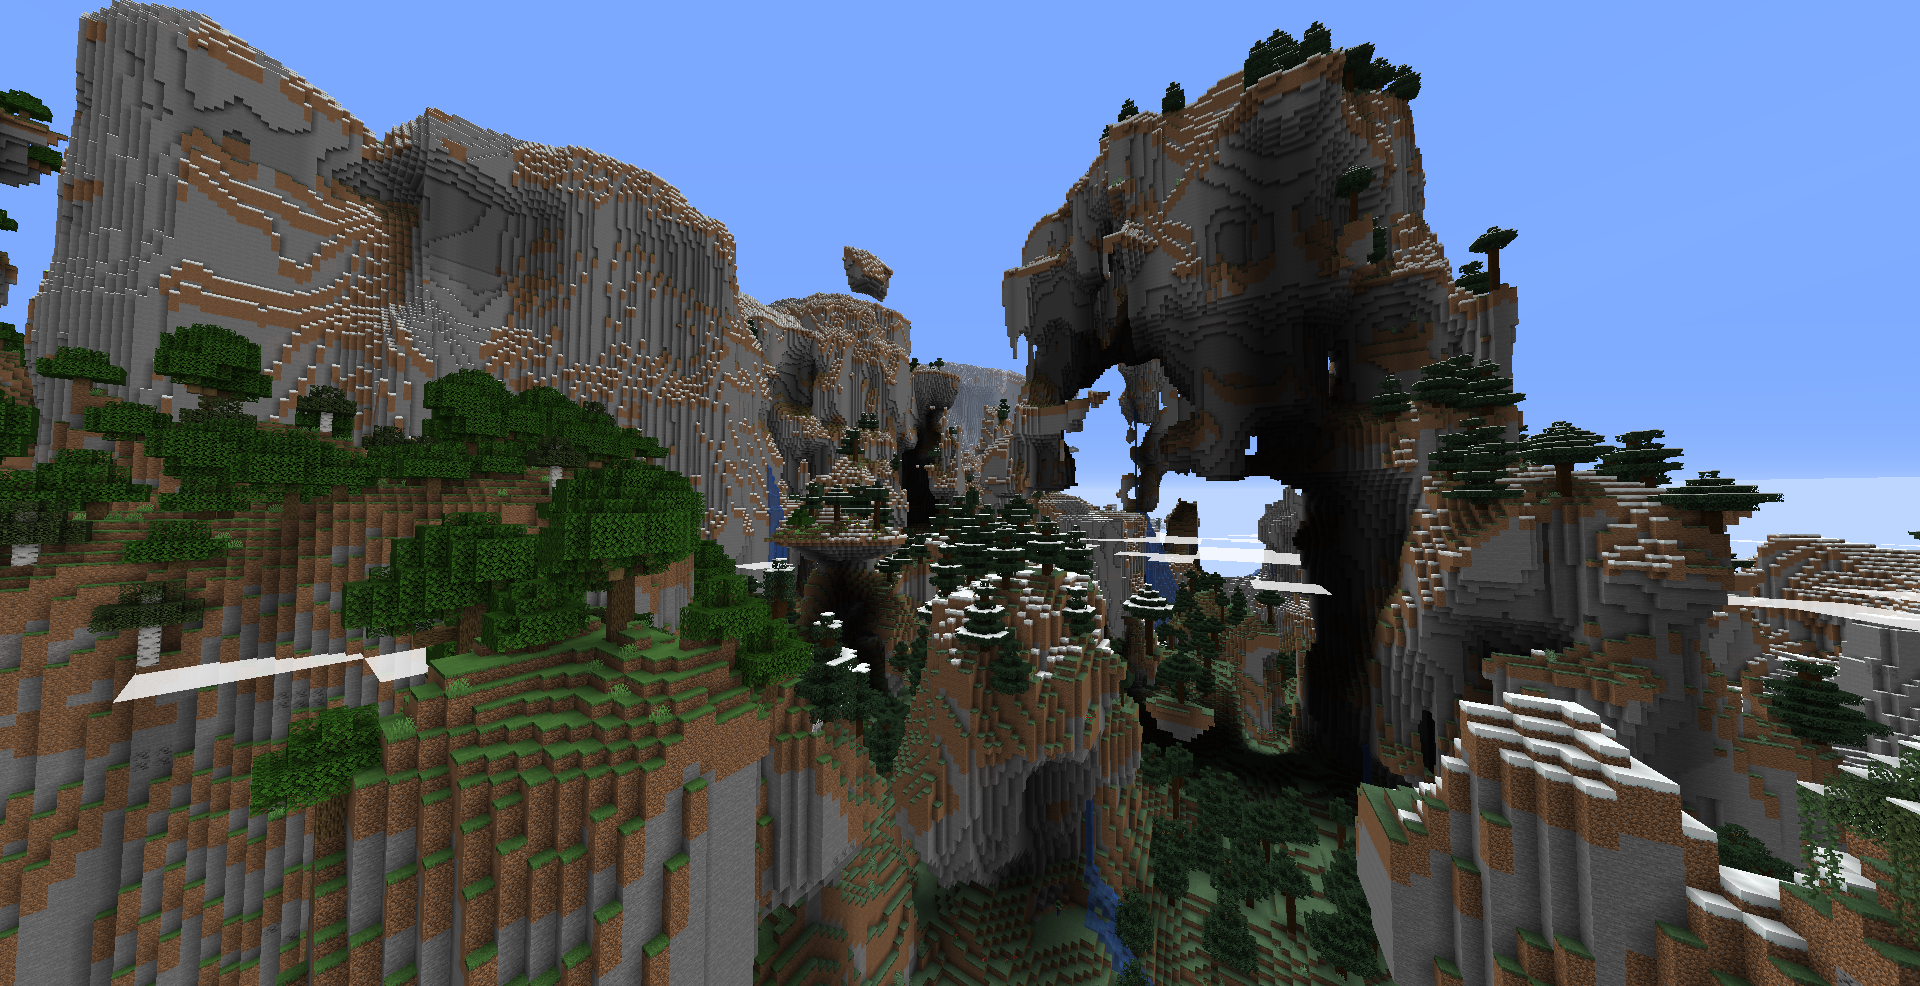
\includegraphics[width=1\linewidth]{Planning report/images/minecraft2.png}
  \caption{Amplified world in Minecraft}
\end{subfigure}
\caption{Screenshots of Minecraft.}
\label{fig:2_minecraft}
\end{figure}

\begin{figure}[H]
    \centering
    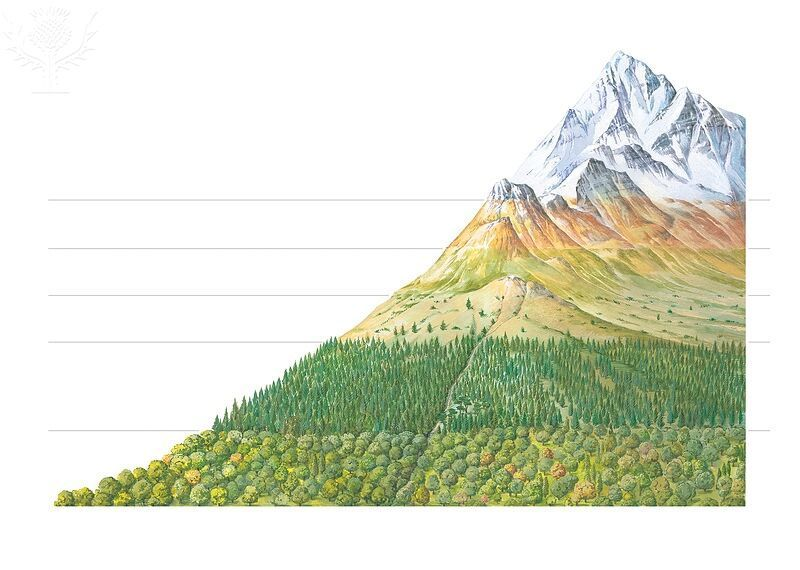
\includegraphics[width=0.5\linewidth]{Planning report/images/biome.jpg}
    \caption{Biome and vegetation altitude zones}
    \label{fig:biome}
\end{figure}


%It is a valid theory that the random generation of worlds using PCG has something to do with the game's overwhelming success.


%Take for example the popular game Minecraft [32], where players find themselves in a world made of three-dimensional cubes of earth, wood, lava and other materials. First steps usually include punching at a tree to obtain some wood, which is then used to build tools to mine other blocks. While it is technically possible to beat the game by defeating an end boss, most players entertain themselves with building structures and obtaining stuff from the world. There are enemies in the game, and other environmental hazards that can kill the player’s avatar, but it is possible to largely avoid violence and focus on building interesting structures


%A few examples of games using PCG are \textit{Diablo} for generating maps, \textit{Spore} for creature animations and \textit{Minecraft} for landscapes and caves \cite[p. 5]{shaker2016procedural}. Perhaps the greatest example of a game utilizing PCG is \textit{No Man's Sky}, which procedurally generates everything from vegetation and creatures to landscapes and planets and thus creates a virtually endless and unique universe for its players to explore \cite{MIT_No_Mans_Sky}.

%As of May 2019 and after 10 years of its official release, \textit{Minecraft} has sold over 176 million copies \cite{Minecraft_10ys}. It is a valid theory that the random generation of worlds using PCG has something to do with the game's overwhelming success.


% skriva mer om grids och cul de sac 

% hur pcg används i andra syften än spel